\section{Theoretical Background}

This chapter provides an overview of base concepts regarding semantic aware vector space representations and neural machine learning models to produce them. Furthermore, we briefly introduce the concept of linguistic dependency types.

\subsection{Evaluation of Semantic Awareness} \label{subsec:eval_semantic_awareness}
Following the Distributional Hypothesis \autocite{sahlgren_distributional_2008,harris_distributional_1954}\todo{AB:check references}, that linguistic items with similar distributions have similar meanings, a conceptional space should be arranged in a way, that distances of concepts follow the human intuition. By doing so, the meaning of these concepts should be as expected as by humans.

We define semantic awareness as a property describing how much meaning a representational space is able to convoy with respect to the space of origin, textual natural language. Furthermore, the state of being semantically aware references the maximal achievable semantic awareness, i.e. convoying the same meaning as the origin of the representation. % move (<-) to previous chapter?

With regard to the Distributional Hypothesis semantic awareness can be measured by the correlation of the distances between different concepts in the representational space and the distances between its source concept representations in the original space. Despite the concept of \textit{distance} seems to be more intuitive in the context of representational spaces, its inverse, the concept of \textit{similarity}, commonly serves as base of comparison.  

Taking similarity measures in both spaces for granted, that map into the same space $X \subseteq \mathbb{R}$, we can borrow the task of \textit{similarity prediction} \todo{AB:add ref} for evaluation of semantic awareness when using \textit{semantic relatedness} as underlying similarity metric of $X$. With the concept of semantic relatedness we refer to the interpretation by \textcite{budanitsky_evaluating_2006}: \textit{linked by any kind of lexical or functional association}. \textcite{resnik_semantic_1999} visualizes this concept by contrasting it with \textit{semantic similarity}. The authors state that "car" and "gasoline" are related, but not semantic similar, whereas "car" and "bicycle" are semantic related \textit{and} similar. Thus, semantic similarity covers only a subset of semantic relatedness and captures relations like synonymy or hypernymy while semantic relatedness further captures antonomy, meronymy and others.

The capability of predicting this kind of similarity in a conceptional space by using an internal representation requires by definition a degree of semantic awareness of this internal space, that we are going to evaluate.

%The distance should not be interpreted as the inverse of semantic similarity, but of semantic \textit{relatedness}. As \textcite{budanitsky_evaluating_2006} highlight, semantic similarity is a specific kind of relatedness (the same applies to antonymy, entailment and others). Therefore, measuring semantic relatedness covers semantical awareness in a more general and accurate way \todo{UL:evidence? Ref!} than other textual comprehension tasks like recognizing textual entailment (RTE)\todo{UL:Ref}, for instance. 

%When we use the sole term \textit{similarity} in the following, we do not reference semantic similarity, but semantic relatedness, like in the common literature about semantic \ac{NLP}.     

\subsubsection{Similarity Prediction}
%In the context of \ac{NLP} 
The task of Similarity Prediction can be framed as to predict a score given two entities of a conceptional space, where higher scores represent higher degrees of similarity between them. In the context of \ac{NLP} these entities are textual documents. The score can model different granularities of similarity, ranging from binary classification, e.g. in the case of Paraphrase Detection\footnote{Paraphrase Detection is the task of identifying if two phrases paraphrase each other.}, weighted aggregation of multi-label classification results, e.g. for instances of discrete %Likert-scaled 
questionnaire data, to regression with continuous scores. 
%Considering its more general nature and the availability of 5-point Likert-scored evaluation data, we will focus on Similarity Prediction as regression task.

We will focus on Similarity Prediction as regression task as it models semantic relatedness based similarity more accurate then binary classification. Semantic Relatedness of arbitrary\footnote{The composition is surely constrained by grammar, linguistic performance and other criteria, but this term is in favor of the tremendous variability of natural language.} composed textual entities is no binary phenomena. Otherwise the entity space would disintegrate into distinct clusters each containing similar entities consequently interpreted as identical. As semantic relatedness is defined about \textit{any} kind of lexical or functional association, it is expected that any entity is semantical related with the majority of the entities in the space in a transitively manner allowing only the trivial solution, precisely, that all entities are identical with respect to the similarity.
The compensation of this fact increases the amount of necessary data to approximate the real behavior. Furthermore, modeling Similarity Prediction as regression is straightforward compared to aggregation of multi-classification output.  

\subsubsection{Evaluation Measures} \label{sec:eval_measures}
Common measures for evaluation of regression estimators are \textit{\acl{MSE}}\todo{UL:ref}, \textit{Pearson correlation coefficient} \autocite{pearson_note_1895} and \textit{Spearman's rank correlation coefficient} \autocite{spearman_proof_1904}.

The \acf{MSE} measures the deviation of the predicted values to the correct ones. It incorporates the variance and the bias of the estimator. A value of zero denotes a perfect estimator and larger values indicate lower estimator performance. Given $n$ predictions $Y$ and corresponding correct values $X$, the \ac{MSE} is defined as follows:
\begin{equation} \label{eq:eval_measure_mse}
MSE = \frac{1}{n}\displaystyle\sum_{i=1}^{n} (Y_i - X_i)^2
\end{equation}

The Pearson correlation coefficient (Pearson's $r$) expresses the degree of linear correlation of two variables. It is the covariance of the variables normalized by their standard deviations. It ranges from $-1$, denoting perfect negative correlation, to $1$, denoting perfect positive correlation. A value of zero expresses that the two variables do not correlate at all. Therefore, higher values above zero indicate better estimator performance. Given $X$ and $Y$, Pearson's $r$ is defined as:
\begin{equation}
r = \frac{\sum_{i=1}^{n}(X_i - \overline{X})(Y_i - \overline{Y})}{\sqrt{\sum_{i=1}^{n}(X_i - \overline{X})^2 \cdot \sum_{i=1}^{n}(Y_i - \overline{Y})^2}} = \frac{Cov(X, Y)}{\sigma(X) \sigma(Y)},
\end{equation}
where $\overline{X}$ is the empirical mean of $X$, $Cov(X, Y)$ is the empirical covariance of $X$ and $Y$, and $\sigma(X)$ is the empirical standard deviation.
%\begin{equation}
%\overline{X} = \frac{1}{n}\displaystyle\sum_{i=1}^{n} X_i;\quad %\text{analogously } \overline{Y}. 
%\end{equation}

Spearman's rank correlation coefficient (Spearman's $\rho$) serves as another correlation based measure, which does not assume linear dependence between $X$ and $Y$. Hence, it is more robust regarding outliers. Spearman's $\rho$ can be interpreted as special case of Pearson's $r$ where the data is converted into ranks before calculation of Pearson's $r$. Given $X$ and $Y$, Spearman's $\rho$ is defined as:
\begin{equation}
\rho = \frac{\sum_{i=1}^{n}(rg(X)_i - \overline{rg(X)})(rg(Y)_i - \overline{rg(Y)})}{\sqrt{\sum_{i=1}^{n}(rg(X)_i - \overline{rg(X)})^2 \cdot \sum_{i=1}^{n}(rg(Y)_i - \overline{rg(Y)})^2}} = \frac{Cov({rg(X)}, {rg(Y)})}{\sigma({rg(X)})\sigma({rg(Y)})},
\end{equation}
where $rg(X)$ are the ranks of $X$. 

%\begin{itemize}[label=]
%\item $rg(X_i)$ is the rank of $X_i$,
%\item $\overline{rg}_X$ is the mean of the ranks of $X$,
%\item $\sigma_{{rg}_X}$ is the standard deviation of the ranks of $X$, and
%\item $Cov({rg}_X, {rg}_Y)$ is the covariance of the ranks of $X$ and $Y$.
%\end{itemize}

\subsection{Artificial Neural Networks}
An \ac{ANN} is a machine learning model where input vectors are mapped to predictions by successive application of computational \textit{layers} \autocite{rumelhart_parallel_1986}. Each layer is a differentiable function $l^{(i)}: \mathbb{R}^{n^{(i-1)}} \mapsto \mathbb{R}^{n^{(i)}}$, with $n^{(i)}$ denoting the size of the input vector for the $i$-th layer, its \textit{layer size}. The arrangement of the layers form the network graph, which is a directed graph defining the specific network architecture. Provided adequate training data, \ac{ANN}s can be trained efficiently with gradient descent based optimization algorithms. In the next sections we will describe some popular architectures and important components of \ac{ANN}s. 

\subsubsection{Feedforward Networks}
The simplest class of \ac{ANN}s are \acl{FNN}s (\acs{FNN}s) that emerged from multilayer Perceptrons \autocite{rosenblatt_perceptron_1958}. Their network architecture forms an acyclic graph and is defined by $f^{FNN}(v) = (l^{(N)} \circ ... \circ l^{(i)} \circ ... \circ l^{(1)})(v)$ where $N$ is the total amount of layers. The $N$-th layer is called \textit{output layer}, all other layers are \textit{hidden layers}. In addition, the virtual \textit{input layer} models the input. Figure~\ref{fig:1} \autocite{epelbaum_deep_2017} shows such a structure. 

%% graphic taken from tomepel/Technical_Book_DL
\begin{figure}[h]
\begin{center}
\begin{tikzpicture}[shorten >=1pt,-stealth,draw=black!50, node distance=\layersep]
    \tikzstyle{every pin edge}=[stealth-,shorten <=1pt]
    \tikzstyle{neuron}=[circle,draw=black,fill=black!25,minimum size=17pt,inner sep=0pt]
    \tikzstyle{input neuron}=[neuron, fill=gray!50];
    \tikzstyle{output neuron}=[neuron, fill=gray!50];
    \tikzstyle{hidden neuron}=[neuron, fill=gray!50];
    \tikzstyle{annot} = [text width=4em, text centered]

    % Draw the input layer nodes
    \foreach \name / \y in {1}
       	\pgfmathtruncatemacro{\m}{int(\y-1)}
    % This is the same as writing \foreach \name / \y in {1/1,2/2,3/3,4/4}
        \node[input neuron, pin=left:Bias] (I-\name) at (0,-\y) {$h_{\m}^{(0)}$};


    \foreach \name / \y in {2,...,6}
       	\pgfmathtruncatemacro{\m}{int(\y-1)}
    % This is the same as writing \foreach \name / \y in {1/1,2/2,3/3,4/4}
        \node[input neuron, pin=left:Input \#\m] (I-\name) at (0,-\y) {$h_{\m}^{(0)}$};

    % Draw the hidden layer 1 nodes
    \foreach \name / \y in {1,...,7}
    	\pgfmathtruncatemacro{\m}{int(\y-1)}
        \path[yshift=0.5cm]
            node[hidden neuron] (H1-\name) at (\layersep,-\y cm) {$h_{\m}^{(1)}$};

    % Draw the hidden layer i node
    \foreach \name / \y in {1,...,6}
        \pgfmathtruncatemacro{\m}{int(\y-1)}
        \path[yshift=0.0cm]
            node[hidden neuron] (H2-\name) at (2*\layersep,-\y cm) {$h_{\m}^{(i)}$};

    % Draw the output layer node
    \foreach \name / \y in {1,...,4}
        \path[yshift=-1.0cm]
    node[output neuron,pin={[pin edge={->}]right:Output \#\y}] (O-\name) at (3*\layersep,-\y cm) {$h_{\y}^{(N)}$};

    % Connect every node in the input layer with every node in the
    % hidden layer.
    \foreach \source in {1,...,6}
        \foreach \dest in {2,...,7}
            \path (I-\source) edge (H1-\dest);

     \foreach \source in {1,...,7}
       \foreach \dest in {2,...,6}
           \path (H1-\source) edge (H2-\dest);

    % Connect every node in the hidden layer with the output layer
    \foreach \source in {1,...,6}
       \foreach \dest in {1,...,4}
          \path (H2-\source) edge (O-\dest);

    % Annotate the layers
    \node[annot,above of=H1-1, node distance=1cm] (hl) {Hidden layer 1};
    \node[annot,left of=hl] {Input layer};
    \node[annot,right of=hl] (hm) {Hidden layer $i$};
    \node[annot,right of=hm] {Output layer};

    \node at ((1.5*\layersep,-3.5 cm) {$\bullet\bullet\bullet$};
    \node at ((2.5*\layersep,-3.5 cm) {$\bullet\bullet\bullet$};
\end{tikzpicture}
\caption{\label{fig:1}Neural Network with $N+1$ layers ($N-1$ hidden layers).}
\end{center}
\end{figure}

There exists a diverse landscape of different types of layers. A common instance is the \ac{FC}. It connects every node from the previous layer with every node from the current one in the term of a weighted sum. Hence, it calculates an affine transformation of its input. Usually a layer $l^{(i)}$ is parametrized by $\theta^{(i)}$, e.g. a set of \textit{weights} and \textit{biases}. In this manner, the \ac{FC} can be defined as:
\begin{equation}
l^{FC}(v;\theta^{(i)}) = w^{(i)}v+b^{(i)} 
\end{equation}
where $w^{(i)} \in \mathbb{R}^{n^{(i)} \times n^{(i-1)}}$, $b^{(i)} \in \mathbb{R}^{n^{(i)}}$ and $\theta^{(i)}=\{w^{(i)}, b^{(i)}\}$. 

\subsubsection{Activation Functions}
The \ac{FNN} described so far is capable of modeling linear mappings only. To enable non-linearity, different non-linear activation functions are applied element-wise to the individual layer outputs. A prominent instance is the \textit{sigmoid} function that takes a real-valued input and "squashes" it to range between 0 and 1. Therefore, it is used to model Bernoulli-Distributions. It is defined as:
\begin{equation}
\sigma(x)=\frac{1}{1+e^{-x}}
\end{equation}

The \textit{hyperbolic tangent} is another strictly increasing activation function, but maps into the range between -1 and 1:
\begin{equation}
\tanh(x)=\frac{1-e^{-2x}}{1+e^{-2x}}=2\sigma(2x)-1
\end{equation}

Finally, the \textit{softmax} function can be used to model discrete probability distributions, e.g. for classification tasks. In contrast to the previous activation functions it is not element wise independent, since it applies normalization across all input elements to guarantee that its result follow the probability distribution conditions. For an input vector $x$ with entries $x_i$ it is defined as:
\begin{equation}
softmax(x_i) = \frac{e^{x_i}}{\sum\limits_{x_j \in x}e^{x_j}} 
\end{equation}

\subsubsection{\acl{RNN}s}
\acl{RNN}s (\acs{RNN}s) introduced by \textcite{hopfield_neural_1982} are \ac{ANN}s that are capable of processing arbitrary long sequences when feeding them stepwise into the network. Especially, they can access information from any previous step and, hence, process the new data conditionally. This is possible via a feedback loop in a \textit{recurrent layer}. Given a sequence of $\tau$-sized vectors $v^{(1)}, ..., v^{(\eta)}$ the $t$-th output $h^{(t)}$ of a recurrent layer $l^{RNN}$ is defined as:
\begin{equation} \label{eq:rnn}
h^{(t)} = l^{RNN}(v^{(t)};\theta) = g(v^{(t)}; h^{(t-1)};\theta)
\end{equation}
where $k, \vartheta \in \mathbb{N}$, $k$ is the inner state size and $g$ is the \ac{RNN} cell function with $g:(\mathbb{R}^\tau; \mathbb{R}^k; \mathbb{R}^\vartheta) \mapsto \mathbb{R}^k$.

The \acf{LSTM} \autocite{hochreiter_long_1997} is a prominent \ac{RNN}. It is a \textit{gated} \ac{RNN}, meaning its cell function $g^{LSTM}$ consists of multiple interconnected gating functions and, further, models a dedicated cell state $\tilde{c}$. \ac{LSTM}s tackle one major draw back of the \ac{RNN} architecture, namely the vanishing gradient problem that occurs when training with long sequences. Without gating, repeated application of one \ac{RNN} cell to the elements of a sequence leads to exponential decrease of the calculated gradients because common activation functions produce gradients lesser 1 that are multiplied according the chain rule. That effect practically hinders the network to use long-distance information. Section~\ref{subsec:gradient_optimization} explains the exact role of gradients in neural network training.

The different gates of the \ac{LSTM} are responsible for deciding what information should be forgotten ($g_f$), which new information will be added ($g_i$) and, finally, which information from $\tilde{c}$ will be presented as output ($g_o$):

\begin{equation} \label{eq:lstm_interm}
\begin{split}
g_f^{(t)} & = \sigma(l^{FC}([\tilde{h}^{(t-1)}, v^{(t)}]; \theta^{(f)})) \\
g_i^{(t)} & = \sigma(l^{FC}([\tilde{h}^{(t-1)}, v^{(t)}]; \theta^{(i)})) \\
g_o^{(t)} & = \sigma(l^{FC}([\tilde{h}^{(t-1)}, v^{(t)}]; \theta^{(o)})) \\
c^{(t)} & = tanh(l^{FC}([h^{(t-1)}, v^{(t)}]; \theta^{(c)})) \\
\tilde{c}^{(t)} & = g_f^{(t)} \odot \tilde{c}^{(t-1)} + g_i^{(t)} \odot \tilde{c} \\
\tilde{h}^{(t)} & = g_o^{(t)} \odot tanh(\tilde{c}^{(t)})
\end{split}
\end{equation}
and finally
\begin{equation} \label{eq:lstm}
g^{LSTM}(v^{(t)};[\tilde{c}^{(t-1)}, \tilde{h}^{(t-1)}]) = [\tilde{c}^{(t)}, \tilde{h}^{(t)}]
\end{equation}
where $[a, b]$ is the concatenation of the vectors $a$ and $b$, and $a \odot b$ denotes their element-wise  product (Hadamard product). We omit the parameter set $\theta^{LSTM} = \{\theta^{(f)}, \theta^{(i)}, \theta^{(o)}, \theta^{(c)}\}$ for better readability.

\subsection{Supervised Training of ANNs}
%In this section we describe the optimization procedure for \acl{ANN}s, e.g their training. 
Supervised training of a model $f$ parametrized by $\theta$ takes a set $\Omega$ of input-output training tuples $(x,y)$ for granted and tries to find instantiations of $\theta$ in the manner that $f(x;\theta) = \hat{y} \approx y, \forall (x,y) \in \Omega$ \autocite{mohri_foundations_2012}. In the context of \ac{ANN}s, one usually uses a \textit{cost function} $J$ that quantifies the deviation of $\hat{y}$ from $y$. $J$ is used to guide the parameter adjustment via gradient-based optimization. 

\subsubsection{Cost Function}
\label{subsec:cost_function}
A cost function, or \textit{loss function}, commonly used for regression tasks is \acf{MSE} as described in section~\ref{sec:eval_measures} because it complies to the maximum likelihood of $y$ and $\hat{y}$ \todo{AB:add ref?} if the error is normally distributed and is efficient to calculate in particular. We reformulate equation~\eqref{eq:eval_measure_mse} to fit into our needs:
\begin{equation}
J^{MSE}_\Omega(\theta) = \frac{1}{n}\sum_{i=0}^{n-1}\sum_{j=0}^{\iota-1}(y_{ij}-\hat{y}_{ij})^2 \label{eq:j_mse}
\end{equation}
where $n$ is the amount of tuples $(x_i, y_i)$ in $\Omega$ and $\hat{y}_i = f(x_i;\theta)$ with $y_i, \hat{y_i} \in \mathbb{R}^\iota$. Note that, despite the cost function depends on the training samples, these are considered to be fixed. 

\subsubsection{Gradient-based Optimization} \label{subsec:gradient_optimization}
Assuming the loss function $J_\Omega$ is differentiable, in theory it would be possible to calculate its global minimum $\theta^*$ analytically. However, in fact that is infeasible for common amounts of parameters in $\theta$ that can be in the order of millions or billions.\todo{UL:evidence, ref}  
%that requires to determine the gradients $\triangledown J_\Omega$ according to all entries in $\Omega$ which is infeasible for large training sets.

Gradient-based optimization tackles this problem by shifting the parameters $\theta$ stepwise in the negative direction of its gradients $\triangledown J_\Omega$. By definition of gradients, an infinitesimal displacement of $\theta$ in this direction decreases $J_\Omega(\theta)$. Hence, we select the parameters for the next optimization step $\theta'$:
\begin{equation}
\theta' = \theta - \alpha\triangledown J_\Omega(\theta)
\end{equation}
where $\alpha$ is the chosen step size, or \textit{learning rate}, that has to be sufficiently small. On the other hand, it is unfavorable to choose a step size too small because that increases convergence time, meaning it slows down training. A lot of different approaches exist that apply dynamical sized stepping like \textit{Momentum} \autocite{polyak_methods_1964}, which takes previous parameter updates into account, or \textit{AdaDelta} \autocite{zeiler_adadelta_2012} that tracks individual learning rates for the parameters in $\theta$. ADAM \autocite{kingma_adam_2014} is another robust method to guide the parameter optimization, it keeps track of the gradients and its square roots.   

As equation \eqref{eq:j_mse} states, one update step requires summation over all training examples in $\Omega$, so it is an $O(n)$ operation\todo{really? not higher?}. Hence, with large training sets calculation of $\triangledown J_\Omega(\theta)$ for every step becomes infeasible. \ac{SGD} addresses this problem by randomly partitioning $\Omega$ into subsets $\Omega^P_i$ of size $n^B$ that are used successively to calculate new parameter sets $\theta'$. Exhausting all $\Omega^P_i$, also referred to as \textit{(mini-)batches}, of a certain partition $\Omega^P$ is called finishing an \textit{epoch}. This approach stochastically approximates the calculation of $\triangledown J_\Omega(\theta)$.

Finally, we describe the core algorithm that enables gradient-based training of \ac{ANN}s, namely \textit{Backpropagation} \autocite{rumelhart_learning_1988}. It uses dynamic programming for efficient calculation of the gradients by exploiting their interconnectivity as present in common \ac{ANN}s. As stated before, an \ac{ANN} $f$ can be represented as a composition of layer functions $l^{(i)}$ with $f(v) = (l^{(N)} \circ ... \circ l^{(i)} \circ ... \circ l^{(1)})(v)$ and $l^{(i)}(v^{(i)}) = v^{(i+1)}$. Hence, the \textit{chain rule} of gradient computation defines the derivatives for two successive layers as:  
\begin{align}
  \frac{dv^{(i+2)}}{dv^{(i)}} & = \frac{dv^{(i+2)}}{dv^{(i+1)}}\frac{dv^{(i+1)}}{dv^{(i)}} \label{eq:chain_1}\\
    & = l^{(i+1)'}(v^{(i+1)})l^{(i)'}(v^{(i)}) \label{eq:chain_2}\\
    & = l^{(i+1)'}(l^{(i)}(v^{(i)}))l^{(i)'}(v^{(i)})  \label{eq:chain_3}
\end{align}
$v^{(i)}$ occurs several times in equation \eqref{eq:chain_3}. Furthermore, as shown in \eqref{eq:chain_1} $\frac{dv^{(i+2)}}{dv^{(i)}}$ depends on $\frac{dv^{(i+2)}}{dv^{(i+1)}}$ immediately. Backpropagation exploits these redundancies by successively calculating all $v^{(i)}$ in a \textit{forward pass}. Then, it calculates all gradients in reverse order while reusing intermediate results in a \textit{backwards pass}. By doing so, the algorithm reduces the complexity from exponential, considering a naive approach, to linear with regard to the edge count of the network graph.

\subsection{A Model for Similarity Prediction}
We divide similarity prediction with regard to textual inputs into transformation of the inputs into vector space representations and 
%similarity measure application. 
similarity calculation in this embeddings space.
%Similarity prediction with regard to textual inputs can be divided into transformation of the inputs into vector space representations and similarity measure application.

\subsubsection{Vector Space Embeddings}
We define \textit{embeddings} of documents, words or other linguistically motivated units as vector space representations that are to a degree semantically aware. Furthermore, \textit{embedding models} are functional transformations that map these units into this \textit{embedding space}. \todo{UL:ref, expand!}

Because of the relevance of embedding models for many \ac{NLP} tasks, a diverse landscape of different approaches has evolved. In the following, we distinguish traditional document embedding approaches from composition based models. By traditional approaches we refer to models which process sequences of opaque tokens and directly produce embeddings for these sequences, whereby composition based models initially embed each token independently and compose these token embeddings into a final vector space representation. \todo{UL: REFS!}  

\subsubsection{Traditional Document Embeddings}
\label{subsec:doc_embedding}
\todo{AB:name Vector Space Models!} XXX READ: \autocite{turney_frequency_2010}
As we focus on distributional semantics, we can outline some common features for traditional document embedding models. These models build upon occurrences of terms $T$ in certain contexts $C$. For instance, a word can occur as a term in a document, i.e. its context, or not. We define $T = \{t_1, ..., t_m\}$ as finite set of opaque symbols with $m = |T|$ and the set of contexts $C \subseteq T^*$ 
% = \{c_1, ..., c_n: c_i = (t \in T)\}$ 
with $n = |C|$, e.g. every context is a sequence of terms. 
The set of unique terms $T$ is called a vocabulary\todo{call it alphabet?}.
%T is called a \textit{vocabulary}.
%Furthermore, we restrict that $\forall C_j \in C: C_j \neq \emptyset$ and $\forall T_i \in T, \exists C_j \in C: T_i \in C_j$. In other words, there are no empty contexts in $C$ and every term in $T$ exists at least in one context of $C$. 
We define a \textit{context embedding} as a function $f_C:C \mapsto \mathbb{R}^{\hat{n}}$, where $\hat{n} \in \mathbb{N}$ is the  dimensionality of the embedding vectors. 

One popular embedding model is based on the \ac{TF-IDF} measure. \ac{TF-IDF} was introduced as \textit{term specificity} in \textcite{sparck_jones_statistical_1972}. Given $T$ and $C$, the term frequency $tf$ of a certain term $t$ with respect to a context $c$ is defined as the count of occurrences of $t$ in $c$ normalized by the maximum of the term counts in this context:
\begin{equation}
tf(t, c) = \frac{\#(t, c)}{max_{t' \in c}\#(t', c)}
\end{equation}
where $\#(t,c)$ is the frequency of term $t$ in context $c$. The inverse document frequency $idf$ of a term $t$ regarding contexts $C$ is defined as:
\begin{equation}
%idf(T_i) = \frac{N}{\sum_{D:T_i \in D} 1}
idf(t) = \frac{|C|}{|\{c \in C: t \in c \}|}
\end{equation}
Finally, the \acl{TF-IDF} $tf.idf$ is calculated:
\begin{equation}
tf.idf(t, c) = tf(t, c) \cdot idf(t) %& T_i\text{ occurs with }C_j \\ 0 & \text{else} \end{cases}
\end{equation}
Hence, given a corpus containing documents as contexts C of terms T, it is possible to calculate a $|T| \times |C|$ \todo{check order of |T| and |C|} \ac{TF-IDF} matrix $M^{tf.idf}$ with $M^{tf.idf}_{ij} = tf.idf(t_i, c_j)$. The columns of $M^{tf.idf}$ represent embeddings for the contexts, respectively documents. The \ac{TF-IDF} context embedding $f_C^{tf.idf}$, i.e. the \ac{TF-IDF} document representation, is defined as $f_C^{tf.idf} (c_j)= M^{tf.idf} \cdot e_j$ where $e_j$ is the j-th unit vector. In the following we call a matrix $M^x$ whose entries $M^x_{ij}$ quantify in any way the occurrences of term $t_i$ in context $c_i$ an \textit{occurrence matrix}. 
%with $f^x_C (C_j)= M^x \cdot e_j$ an embedding matrix for the embedding $f^x_C$.

Another common approach utilizes \acl{PMI} \autocite{church_word_1990}. \acf{PMI} quantifies the association of two outcomes of discrete random variables $X$ and $Y$. Given outcomes $x$ and $y$ belonging to these variables, the \ac{PMI} is defined as:
%discrepancy between the probability of the coincidence of two events given their joint distribution and their individual distributions, assuming independence. 
%Given the outcomes $x$ and $y$ belonging to discrete random variables $X$ and $Y$, the \ac{PMI} defines the :
\begin{equation}
	pmi(x;y) \equiv log\frac{p(x,y)}{p(x)p(y)}
\end{equation}
By interpreting $T$ and $C$ as random variables $X$ and $Y$ an occurrence matrix $M^{pmi}$ 
%that approximates this behavior 
can be constructed as follows:
\begin{equation}
\begin{split}
M^{pmi}_{ij} & = log\frac{\#(t_i, c_j)}{\sum\limits_{c \in C}\#(t_i, c) \cdot \sum\limits_{t \in T}\#(t,c_j)} \\
 & = log\,\#(t_i, c_j) - b_i^{(T)} - b_j^{(C)}
\end{split}
\end{equation}
where $b_i^{(T)}$ and $b_j^{(C)}$ are term and context biases with
\begin{equation} \label{eq:m_pmi}
\begin{split}
b_i^{(T)} & = log \sum\limits_{c \in C}\#(t_i, c) \quad \text{and} \\
b_j^{(C)} & = log \sum\limits_{t \in T}\#(t,c_j)
\end{split}
\end{equation}

Because $\#(T_i, C_j)$ is zero and, consequently, $M^{pmi}_{ij}$ equals $-\infty$ for a lot of entries, often the \ac{PPMI} \autocite{niwa_co-occurrence_1994} is used:
\begin{equation}
M^{ppmi}_{ij} = max(M^{ppmi}_{ij}, 0)
\end{equation}

By construction these document representations have as many dimensions as unique terms exist in $T$. Bur according to Zipf's Law ... This draw back\todo{UL:explain, why bad -> main argument(?)} can be tackled by filtering very frequently occurring words, called \textit{stop words}, assuming they do not convey particular meaning, and, further, very rare words to handle\todo{UL:explain!} Zipf's word frequency law in natural language\todo{UL:ref}. But even after ...\todo{add content}, the resulting embeddings are very sparse because the majority of words occur only in small subsets of a natural language corpus if the term distributions are not artificially controlled\todo{UL:ref}. %Respectively, a lot of possible word co-occurrences never occur. 

To combat this problem\todo{UL:main argument}, there are several methods to reduce the embedding dimensionality while maintaining semantic awareness. One common approach is to apply \ac{SVD} to the occurrence matrix. \ac{LSA} \autocite{deerwester_indexing_1990} implements this in the context of \ac{IR} by decomposing the occurrence matrix $M$ described above\footnote{The original \ac{LSA} makes use of the \textit{term document matrix} $M^{td}$, a simplification of $M^{pmi}$ without normalization, where $M^{td}_{ij} =\nobreak \#(T_i, C_j)$.}\todo{UL:ref} in the following way:
\begin{equation}
M = U \cdot S \cdot V^T
\end{equation}
where $U = MM^T$, $V = M^TM$ and $S$ is a diagonal matrix that contains the eigenvalues of $M$. Furthermore, $U$ and $V$ are orthogonal bases, whereby $U$ spans a term based vector space and $V$ a document based vector space. Using this, a dimensionality reduction can be done by removing the smallest eigenvalues from $S$ resulting in the submatrix $S_{(\hat{n})}$ that contains only the $\hat{n}$ highest eigenvalues. This is a reasonable step because $S_{(\hat{n})}$ and the corresponding matrices $U_{(\hat{n})}$ and $V_{(\hat{n})}$ produce the rank $\hat{n}$ approximation to $M$ with the smallest error\footnote{according to Frobenius norm}\todo{UL:ref}. Mapping a document representation $d$, where $d$ consists of entries as in $M$, into the reduced dimensional space spanned by $V_{(\hat{n})}$ can be computed by: 
\begin{equation} \label{eq:svd_doc}
\hat{d} = S_{(\hat{n})}^{-1}U_{(\hat{n})}^Td
\end{equation}
where $\hat{d}$ is the $\hat{n}$-dimensional document representation. 

Despite its clear theoretical motivation SVD based\todo{UL: more accurate} VSM\todo{AB:introduce!}s have the major draw back that the decomposition algorithm has to be applied every time a document or a term is added\todo{UL:Wozu?}. \ac{SVD} is computational expensive, it has a complexity of $O((n+m)^2\hat{n}^3)$. Assuming that $T$ does not change as much as $C$, approaches arise that build upon (pre-) calculated \textit{word} or \textit{term embeddings}\todo{UL:ref}. Then, embedded terms are dynamically composed to document representations leading to \textit{composition models}\todo{UL:ref}. We will outline these concepts in the following sections.

\subsubsection{Term Embeddings}
Term embeddings, in their common sense, are distributed representations of words \autocite{bengio_neural_2003}, thus forming \acfp{DSM}\todo{AB:REF}. Similar to context embeddings, we define a term embedding as a function $f_T:T \mapsto \mathbb{R}^{\hat{m}}$, where $\hat{m} \in \mathbb{N}$ is the dimensionality of the resulting embedding vectors.

The methods described in the previous section are directly applicable to produce term embeddings by defining $f_T(t_i) = M^T \cdot e_i$ where $M \in \mathbb{R}^{m \times \hat{m}}$\todo{AB:define or replace $m$} is an occurrence matrix. A common approach to produce term embeddings is to calculate $M^{ppmi}$ and apply \ac{SVD}. In analogy to $\hat{d} = S_k^{-1}U_k^Td$ (equation \eqref{eq:svd_doc}), a term embedding $\hat{t}$ of the context based term vector $t$ of term $T_i$ can be calculated as $\hat{t} = S_k^{-1}V_k^Tt$.\todo{UL:explain benefit!}

Further ideas like the Hyperspace Analogue to Language model \autocite{lund_producing_1996} build upon co-occurrence counts. They can be cast into the conceptional framework outlined by defining $C$ via a co-occurrences relation $R^{CO}$ as:% \subseteq T \times T$ as:
\begin{equation} \label{eq:co}
C_j = \{t_i|(t_i, t_j) \in R^{CO}\}
\end{equation}
where $R^{CO} = \{(t_i, t_j)|t_i, t_j \in T; \text{ $t_i$ and $t_j$ are successive tokens}\}$. This approach can be enhanced by relaxing the co-occurrence relation, e.g. defining $R^{CO}$ via a fixed or soft sized co-occurrence window larger than two and optionally adding distance weighting.\todo{AB:refs?}

In line with \textcite{levy_improving_2015} we refer to the term embedding models presented so far as \textit{count based} models and contrast them with \textit{prediction based} models. Prediction based embedding models commonly are \ac{ANN}s whose intermediate low\footnote{with respect to the size of $T$} dimensional layer results \todo{UL:add figure} are exploited as term embeddings\todo{UL:introduce idea before "how-to"/technical explanation}. They raised attention due to recently published methods that allow efficient embedding calculation with regard to billions of tokens. The \ac{SGNS}\footnote{A \ac{SGNS} implementation was released within the word2vec framework \autocite{mikolov_efficient_2013}.} \autocite{mikolov_distributed_2013} is a popular candidate that does not immediately\todo{UL:UNCLEAR} rely on an occurrence matrix, but trains a simple, one hidden layer \acs{ANN} with the objective to predict the context of a term, e.g. the neighbors of the tokens in a textual corpus. The core Skip-Gram idea can be formalized as:
\begin{equation}
\begin{split}
f^{SG}_T(t_i)_j & = p(c_j|t_i) \\
  & = (softmax \circ l^{FC}_{out} \circ l^{FC}_{hidden})(e_i) \cdot e_j \\
  & = softmax(l^{FC}_{out}(l^{FC}_{hidden}(e_i; \{w_{H};b_{H}\}); \{w_{O};b_{O}\}) \cdot e_j \\
  & = softmax(w_{O}(w_{H} \cdot e_i + b_{H}) + b_{O}) \cdot e_j \\
  & = softmax([w_{O},b^T_{O}] \cdot [w_{H},b^T_{H}]\cdot e_i) 
  \cdot e_j \\
  & = softmax(M^{out} \cdot M^{hidden} \cdot e_i) \cdot e_j
\end{split}
\end{equation}
Then, the Skip-Gram term embedding can be defined as $f_T^{SG}(t_i) = M^{hidden} \cdot e_i$. Although $M^{hidden}$ does not obviously rely on occurrence counts immediately, \textcite{levy_neural_2014} showed that, in fact, Skip-Gram factorizes a shifted \ac{PMI} matrix in the way that: 
\begin{equation}
M^{hidden} \cdot M^{out} + log(k) = M^{pmi}
\end{equation}
where $k$ is a constant. 

Glove \autocite{pennington_glove_2014} is a prediction based model that explicitly uses $M^{pmi}$. Its cost function \todo{UL:introduce! (??)} $J^{GLOVE}$ can be defined as:
\begin{equation}
J^{GLOVE}(\{w; b\}) = \sum\limits_{t_i \in T}\sum\limits_{c_j \in C}\ M^{B}_{ij}(w_i^Tw_j + b_i + b_j - log\,\#(t_i,c_j))^2
\end{equation}
where $M^B$ is a fixed matrix of biases and $|T| = |C|$, i.e. the number of possible terms equals the number of possible contexts. The later is feasible because Glove uses co-occurrences to define $C$ as described in equation \eqref{eq:co}, therefore contexts can be identified by terms.\footnote{The same holds for Skip-Gram.}

If we recap the definition of $M^{pmi}$, $M^{pmi}_{ij}= log\,\#(t_i, c_j) - b^{(T)}_i - b^{(C)}_j$ (see equation \eqref{eq:m_pmi}), we notice that Glove's objective factorizes $M^{pmi}$:%, but using a composed $b$ instead of $b^{(T)}$ and $b^{(C)}$:
\begin{align}
%ww^T & = log\,\#(T_i, C_j) - b_i - b_j \\
% & = M^{pmi}_{ij} + b^{(T)}_i + b^{(C)}_j - b_i - b_j
(w^Tw)_{ij} & = log\,\#(t_i, c_j) - b_i - b_j \\
(w^Tw)_{ij} + b_i - b^{(T)}_i + b_j - b^{(C)}_j & = M^{pmi}_{ij}
\end{align}
\todo{re-write eq:28 into matrix operations (?)}
Note, that, in contrast to Skip-Gram, this approach implements full symmetry with regard to $T$ and $C$. By doing so, all information is accumulated in one mapping, context specific information is not outsourced\todo{UL:unclear!}, like it does the default Skip-Gram model with $M^{out}$\footnote{This can be circumvented for Skip-Gram by using $(f^{SG}_T(t_i) + f^{SG}_C(c_i))$ or $[f^{SG}_T(t_i), f^{SG}_C(c_i)]$ as term embedding for further application, where $f_C^{SG}(c_i) = (M^{out})^T \cdot e_i$.}:\todo{UL: too short! benefit?}
\begin{equation}
f_T^{GLOVE}(t_i) = f_C^{GLOVE}(c_i) = w \cdot e_i + b_i 
\end{equation}

\subsubsection{Composition Models}
\acfp{CDSM} \todo{AB:REF!} intend to produce document embeddings $\hat{d}$ from a sequence of term embeddings $\hat{s} = [\hat{t}_1, ..., \hat{t}_\kappa]$ with $\forall \hat{t} \in \hat{s}: \hat{t} = f_T(t), t \in T, \hat{t} \subseteq \mathbb{R}^{\hat{m}}$. They can be expressed recursively by:
\begin{equation}
\begin{split}
f_{CM}(\hat{s}) & = f_N(f_{Rec}(\hat{s}; h_I); |\hat{s}|) \quad \text{and} \\
f_{Rec}(\hat{s}; h) & = 
  \begin{cases}  
    h & \text{ if }|\hat{s}|=0 \\
    f_{Rec}([\hat{t}_2, ..., \hat{t}_\kappa]; f_R(f_M(\hat{t}_1); h)) & \text{ else}
  \end{cases}
\end{split}
\end{equation}
where $f_M: \mathbb{R}^{\hat{m}} \mapsto \mathbb{R}^{\mathring{m}}$ is the term embedding \textit{mapping function}, $f_R: (\mathbb{R}^{\mathring{m}},\mathbb{R}^k) \mapsto \mathbb{R}^k$ is the internal \textit{reduction function}, $f_N: (\mathbb{R}^k, \mathbb{N}) \mapsto \mathbb{R}^{\hat{n}}$ is a \textit{normalization function} and $h_I \in \mathbb{R}^k$ is the initial internal state.

In the following we distinguish \textit{order unaware} composition models from \textit{order aware} models. Both types commonly use the identity function or $(htan \circ l^{FC})$ as mapping function $f_M$. There are also hybrid approaches based on n-grams and Convolutional Neural Networks\footnote{They fit into the definition of $f_{CM}$ by relaxing $f_M$, which is, in fact, a convolution kernel of size one, to $f_{M_{cnn}}: (\mathbb{R}^{\hat{m}}, ... ,\mathbb{R}^{\hat{m}}) \mapsto \mathbb{R}^{\mathring{m}}$ and using the \textit{max} function for $f_{R_{cnn}}$ to implement max pooling, for instance.}, but these are out of scope for this work.

\subsubsection*{Order unaware composition} 
These models are known as Bag-of-Words models. They can be defined by constraining the reduction function $f_R$ to be associative and commutative. Common instances are \textit{summation} with:
\begin{equation}
f_{R_{sum}}(\mathring{t}; h) = h + \mathring{t} \quad \text{and} \quad h_{I_{sum}} = [0, ..., 0]^T \in \mathbb{R}^k, k = \mathring{m}
\end{equation}
or \textit{averaging} with: 
\begin{equation}
f_{R_{avg}} = f_{R_{sum}}, \quad h_{I_{avg}} = h_{I_{sum}} \quad \text{and} \quad f_{N_{avg}}(\dot{d}; \kappa) = \frac{1}{\kappa} \cdot \dot{d}
\end{equation}

\subsubsection*{Order aware composition} \label{subsec:order_aware_composition}
These models take the ordering of the input tokens into account. Commonly they build upon \acl{RNN}s. So, we can define the reduction function as:
\begin{equation}
f_{R_{rnn}} = g^{RNN}
\end{equation}
where $g^{RNN}$ is an \ac{RNN} cell function (see equation~\eqref{eq:rnn}, assuming $\theta$ is fixed) like $g^{LSTM}$ (see equation~\eqref{eq:lstm}), for instance. As it is commonly known from \ac{RNN} literature \todo{AB: REFS!!}, using these kind of non-associative composition functions leverages \todo{AB: enables?} contextualized processing of the individual tokens.

\subsubsection{Similarity measures}
\label{subsec:similarity_measure}
A similarity measure for embeddings is a symmetric function $f_S: (\mathbb{R}^{\hat{n}}, \mathbb{R}^{\hat{n}}) \mapsto [0, 1] \subset \mathbb{R}$ with:\todo{UL: why not sim(a,a)=1 ?}
\begin{equation}
f_S(\hat{d}_i, \hat{d}_i) \geq f_S(\hat{d}_i, \hat{d}_j)
\end{equation}
The \textit{cosine similarity} is a prominent similarity measure, that is defined by:
\begin{equation} \label{eq:sim_cos}
%\begin{split}
%\frac{\sum_{l=1}^{\hat{n}}\hat{d}_{il} \hat{d}_{jl}}{\lVert\hat{d}_i\rVert_2 \lVert\hat{d}_j\rVert_2} \\
%f_{S_{cos}}(\hat{d}_i, \hat{d}_j) & = \frac{(\hat{d}_{i})^T \cdot \hat{d}_{j}}{\lVert\hat{d}_i\rVert_2 \lVert\hat{d}_j\rVert_2} \\
f_{S_{cos}}(\hat{d}_i, \hat{d}_j) = \frac{\sum_{k=1}^{\hat{n}}\hat{d}_{i_k} \hat{d}_{j_k}}{\norm{\hat{d}_i}_2 \norm{\hat{d}_j}_2} = \left(\frac{\hat{d}_i}{\lVert\hat{d}_i\rVert_2}\right)^T \cdot \frac{\hat{d}_j}{\lVert\hat{d}_j\rVert_2}
%||\hat{d}_i||_2 \cdot ||\hat{d}_j||_2^T
%\end{split}
\end{equation}
where $\norm{v}_2 = \sqrt{\sum_{k=1}^{|v|}(v_k)^2}$ is the $L_2$ (euclidean) norm of $v$. As equation~\eqref{eq:sim_cos} shows this measure explicitly normalizes its input. This can be an advantage because it is independent of the \textit{significance}\todo{UL explain intuitively! not just on the side...} of the embeddings which is, as \textcite{schakel_measuring_2015} state, encoded by their norm.

\todo{AB:throw away?}An \textit{euclidean} \todo{UL:euclidean, in what way?} distance based similarity measure that relies directly on the euclidean norm can be constructed as:
\begin{equation}
f_{S_{eucl}}(\hat{d}_i, \hat{d}_j) = exp(-\lVert\hat{d}_i - \hat{d}_j\rVert_2)
\end{equation}


Similarly, the \textit{manhattan/taxicab} distance can be used as similarity measure as proposed by \textcite{mueller_siamese_2016}:
\begin{equation}
f_{S_{manh}}(\hat{d}_i, \hat{d}_j) = exp(-\lVert\hat{d}_i - \hat{d}_j\rVert_1)
\end{equation}
where $\lVert v\rVert_1 = \sum\limits_{l=1}^{|v|}|v_l|$ is the $L_1$ norm of $v$. Compared with the other measures, $f_{S_{manh}}$ has the lowest calculation costs. %Furthermore, it 

\subsection{Linguistic Dependency Types}
In the following, we present a very brief introduction into the theory of linguistic dependency grammar and typed dependency relations that was mainly distilled from \textcite{jurafsky_dependency_2014}.

\subsection{Dependency Grammar}
\ac{DG} is a class of syntactic theories rooted in the work of Lucien Tesni\`{e}re \autocite{tesniere_elements_1976}. Its formalism describes the structure of sentences by linking individual words in a sentence with each other by directed, binary relations forming a tree commonly rooted by the finite verb. In this manner, any word has zero or multiple \textit{dependents} linked by \textit{dependency} relation instances. With respect to its dependents, a word is referred to as \textit{head}. A head and its dependents mark a linguistic unit in the hierarchical structure. Figure~\ref{fig:displacy_deps} shows an example dependency syntax tree.

\begin{figure}[htb!]
  \centering
  % image workflow (displacy -> this):
  % 1) create svg with https://demos.explosion.ai/displacy/
  % 2) remove POS labels (with text editor)
  % 3) convert to pdf online
  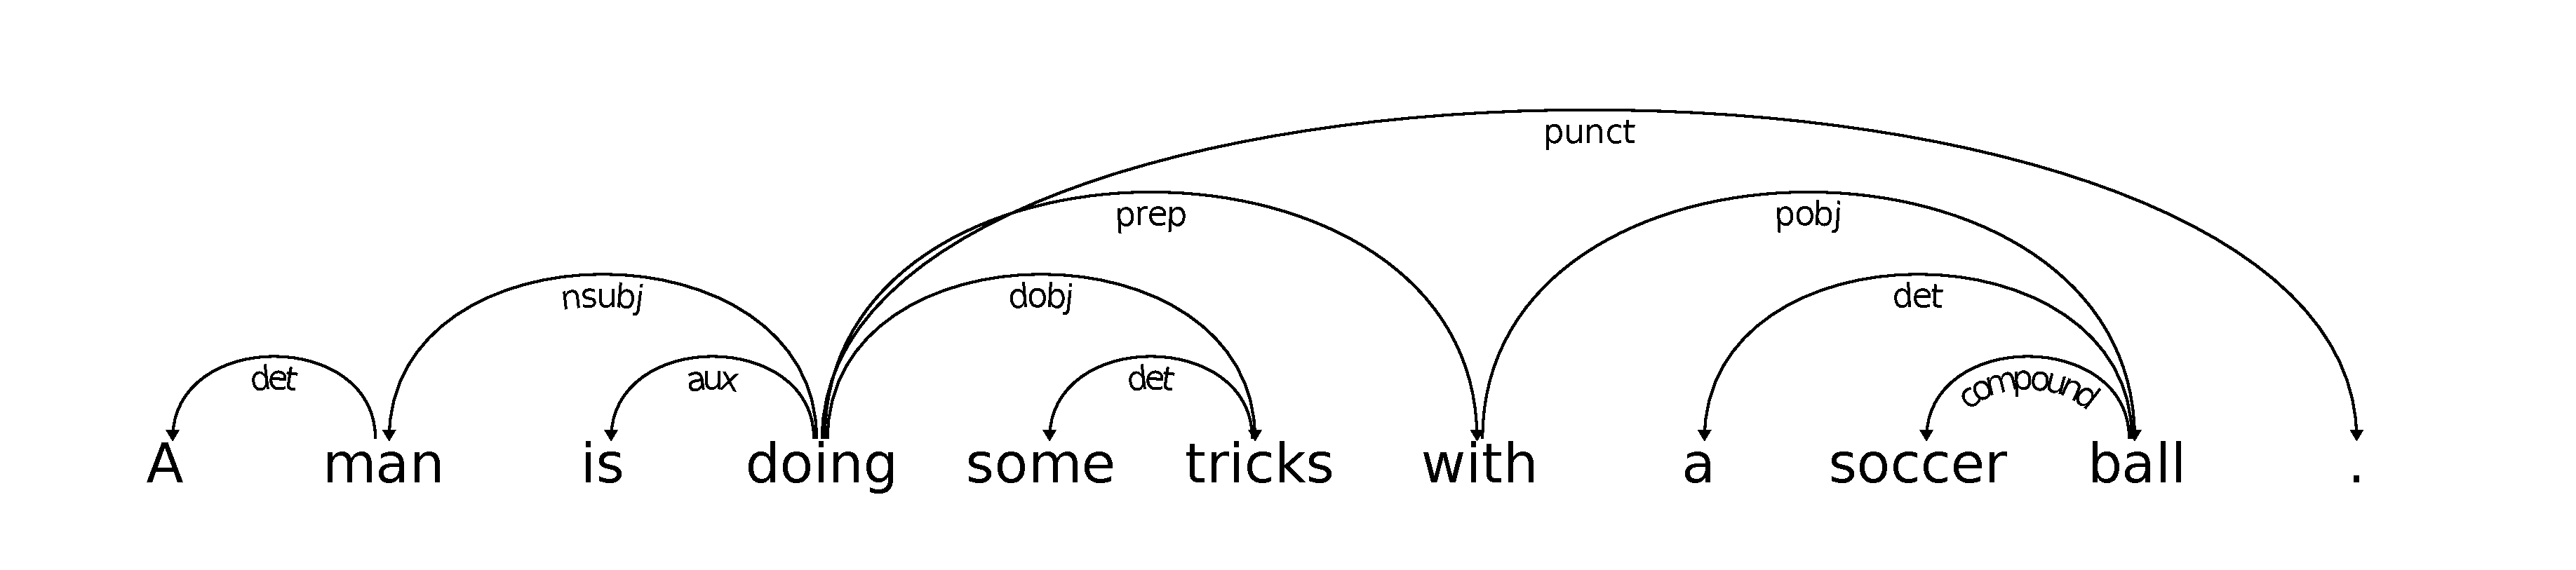
\includegraphics[width=1.\linewidth]{background/depparse_displacy.pdf}
  \caption{Dependency parse tree with typed relations. Arcs point from heads to their dependents. They are labeled with dependency types.}
  \label{fig:displacy_deps}
 \end{figure}


\subsubsection{Dependency Types}
%Dependents modify their head, but a head governs its dependents. 
 %, similar to a linguistic constituent. 
In addition to structural \todo{AB: or hierarchical?} information given by the dependence relation, dependency grammars allow to classify the kinds of dependencies in terms of the grammatical role the dependent plays with respect to its head, e.g. \textit{subject}, \textit{direct object} or \textit{indirect object}. The example roles mentioned are commonly known and relate to the main finite verb. Because they link phrases of clauses, they are kinds of \textit{clausal argument relations}. To classify all types of dependencies found in dependence structures, the \ac{DG} formalism expands the set of grammatical roles further to types of \textit{nominal modifier relations}, \textit{conjunctions} and many others. But languages vary and the amount of explicitly expressed grammatical functions do as well, e.g. morphological rich languages express a lot of functionality implicitly by inflection, that is, otherwise, expressed by grammatical function words. Nevertheless, efforts are being made to standardize the landscape of considered types of dependency relations. One approach that recently gains attention is the Universal Dependencies project \autocite{nivre_universal_2016}. It achieved to determine a common core of 40 grammatical relations while maintaining flexible enough to incorporate language specific types, if needed. The project currently provides resources annotated with dependency structure (treebanks) for 60 different languages.

The English language is more or less restricted in its word order and has weak morphology. As \textcite{jurafsky_dependency_2014} states, in this case, the dependency type strongly correlates with the position of the individual words.


\begin{comment}
\subsection{Transfer Learning}
Successful supervised deep learning depends on access to certain amounts of quality labeled training data. Despite big datasets for some tasks exist by now, that is not every time the case since dataset creation is expensive. However, a lot of tasks and domains share common subsets. Transfer learning aims to exploit these interdependencies by conveying knowledge learned at one domain and task to another. 

Following the notation of \textcite{pan_survey_2010} we define a \textit{domain} $\mathcal{D}$ as $\mathcal{D} = (\mathcal{X}, P(X))$ and a \textit{task} $\mathcal{T}$ as $\mathcal{T} = (\mathcal{Y}, P(Y|X))$ where $\mathcal{X}$ and $\mathcal{Y}$ are feature and label spaces, respectively, $P(X)$ is a marginal probability distribution with $X = \{x_1, ..., x_n\} \in \mathcal{X}$ and $P(Y|X)$ is a conditional probability distribution with $Y = \{y_1, ..., y_m\} \in \mathcal{Y}$\todo{merge notation with previous one}.
Hence, given source and target domains $\mathcal{D}_S$ and $\mathcal{D}_T$ and source and target tasks $\mathcal{T}_S$ and $\mathcal{T}_T$, one can enumerate different qualities of transfer learning:% scenarios/features/qualities(?):
\begin{enumerate}
\item $\mathcal{D}_S \neq \mathcal{D}_T$
\item $P(X_S) \neq P(X_T)$
\item $\mathcal{T}_S \neq \mathcal{T}_T$
\item $P(Y_S|X_S) \neq P(Y_T|X_T)$
\end{enumerate}
where, theoretically, any combination is possible, but usually $(1.) \Rightarrow (2.)$ and $(3.) \Rightarrow (4.)$. 

Training and usage of term embeddings is an instance of transfer learning where conditions $(3.)$ and $(4.)$, and optionally $(2.)$, hold, that is known as unsupervised \textit{feature representation learning}. These and similar approaches in the context of deep learning \autocite{glorot_domain_2011,chen_marginalized_2012}, in fact, implement an \textit{autoencoder} \autocite{bengio_deep_2012}. An autoencoder compresses its input into a small feature vector and tries to reconstruct it from this representation.

\textit{Transductive transfer learning} or \textit{domain adaption} is a scenario where $\mathcal{T}_S = \mathcal{T}_T$, but $P(X_S) \neq P(X_T)$. Taking efficient term embeddings for granted, this work focuses on domain adaption as we examine the effect of pre-training the model on a large corpus based on the PPDB dataset which is further fine-tuned and evaluated on the pertinent domain, the SICK dataset, respectively. 

%domain independence \\
%mixing vs. pre-training/fine-tuning\\
%contrast with multi-task learning \\ 

\end{comment}
